\begin{enumerate}[label=\alph*)]
  \item D'abord on apprend que
  
\begin{verbatim}
help hilb
 HILB   Hilbert matrix.
      HILB(N) is the N by N matrix with elements 1/(i+j-1),
      which is a famous example of a badly conditioned matrix.
\end{verbatim}
  
  On peut calculer les quantités nécessaires avec les commandes suivantes, dans une boucle \texttt{for} pour $n = 1, 2, \dots, 10$: 
  
\begin{verbatim}
for n=1:10
    A = hilb(n);
    KA(n) = cond(A);
end 
\end{verbatim}

  \item Le conditionnement de la matrice $A$ est enregistré dans le vecteur \texttt{KA}, qui vaut
  
        \lstinputlisting{s4/matlab/KA.txt}
  
        et son comportement en fonction de $n$ peut être visualisé avec les commandes suivantes :

\begin{verbatim}
figure(1);
semilogy([1:1:10],KA,'r');
grid;
xlabel('n');
ylabel('K(A)');
\end{verbatim}

      On peut observer à la Figure \ref{fig:KA} que le conditionnement a une comportement linéaire sur le graphique, c'est-à-dire $K_{2}\parent{A}$ croit (presque) exponentiellement en fonction de $n$.
      
      \begin{figure}[h!]
        \centering
        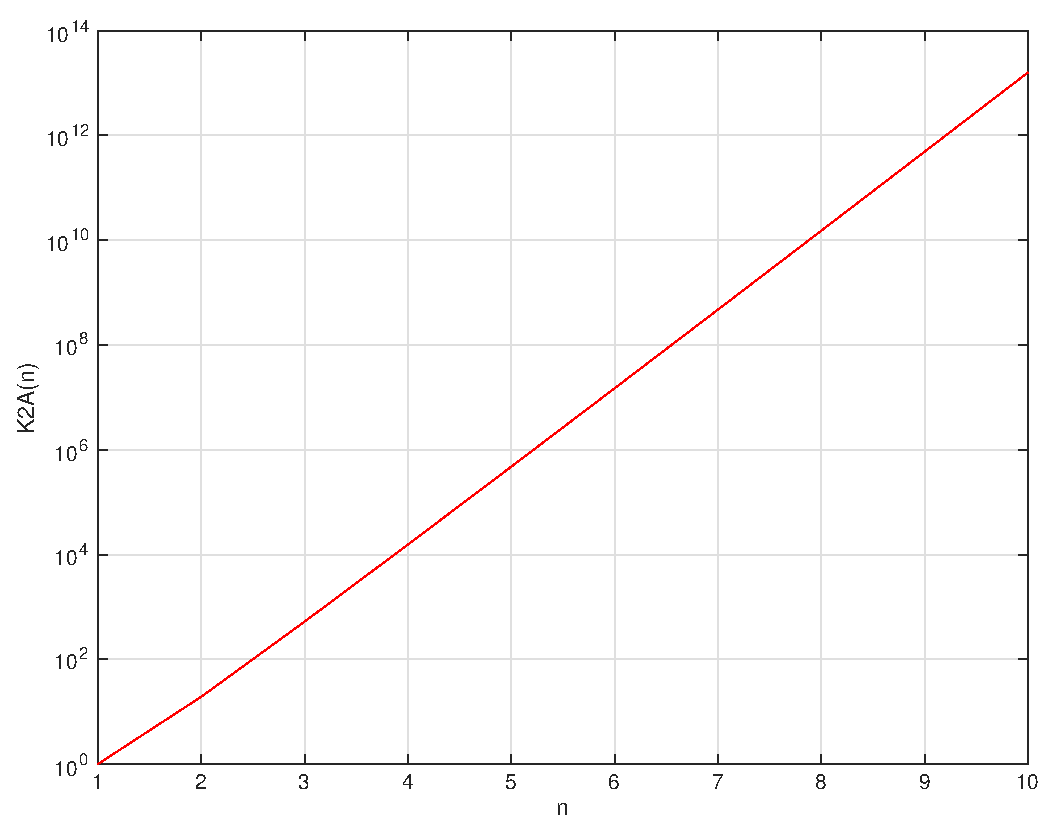
\includegraphics[scale = 0.5]{s4/matlab/KA.eps}
        \caption{Graphique du conditionnement de la matrice de Hilbert en fonction de $n$ ; l'échelle est linéaire sur les abscisses et logarithmique sur les ordonnées.}
        \label{fig:KA}
      \end{figure}

      \item On veut construire un vecteur colonne $\BoldX_{e x}$ aléatoire avec $n$ composantes, calculer le vecteur $\BoldB = A \BoldX_{e x}$, résoudre (pour chaque $n = 1, 2, \dots , 10$) le système linéaire $A \BoldX = \BoldB$ et calculer l'erreur relative

      \begin{equation*}
        \varepsilon^{r} = \dfrac{\norm{\BoldX - \BoldX_{e x}}}{\norm{\BoldX_{e x}}};
      \end{equation*}
      
      on peut utiliser le code suivant :
      
\begin{verbatim}
for n=1:10
    A = hilb(n);
    KA(n) = cond(A);
    xex = rand(n,1);
    b = A * xex;
    x = A\b;
    err(n) = norm(x-xex)/norm(xex);
end
\end{verbatim}

    Ensuite, pour visualiser le comportement du conditionnement et de l'erreur relative $\varepsilon^{r}$ sur le même graphique, on peut taper :
    
\begin{verbatim}
figure(2);
semilogy([1:1:10], KA, 'r', [1:1:10], err, 'h');
grid;
xlabel('n');
ylabel('KA(n) & err(n)');
\end{verbatim}

\begin{figure}[h!]
  \begin{subfigure}[b]{0.5 \linewidth}
    \centering
    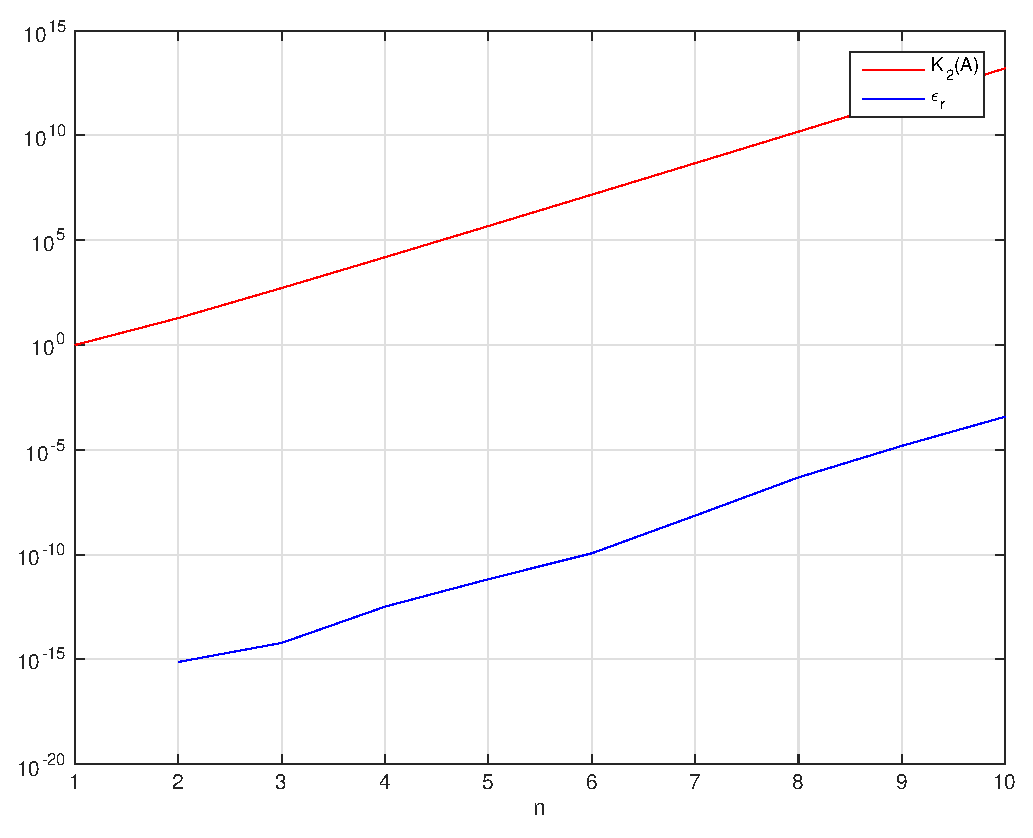
\includegraphics[scale=0.4]{s4/matlab/KVSErr} 
    \caption{$K$ et $\varepsilon^{r}$ en fonction de $n$.} 
    \label{figKAAndErra} 
  \end{subfigure}
  \begin{subfigure}[b]{0.5 \linewidth}
    \centering
    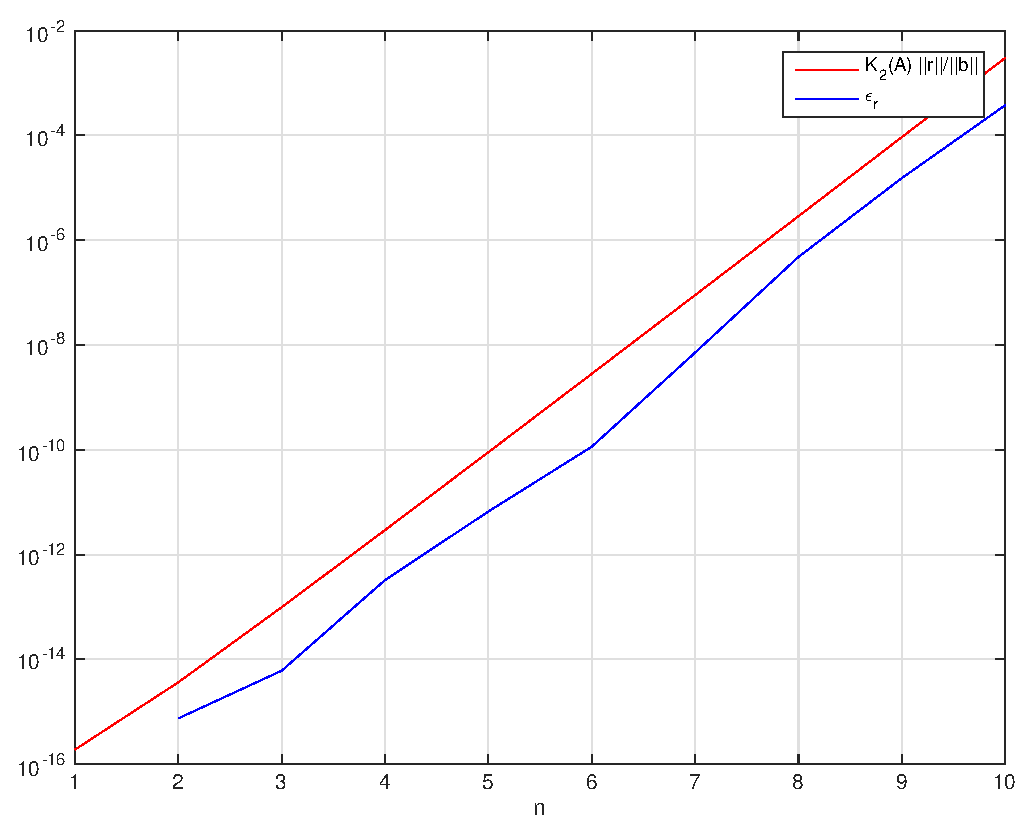
\includegraphics[scale=0.4]{s4/matlab/ErrVSTildeErr} 
    \caption{$\tilde{\varepsilon}^{r}$ et $\varepsilon^{r}$ en function de $n$.} 
    \label{figKAAndErrb} 
  \end{subfigure} 
  \caption{A gauche, Figure 4(a) : Graphique du conditionnement de la matrice de Hilbert, $K$, et de l'erreur relative, $\varepsilon^{r}$, définie à l'équation \eqref{eq:err}, en fonction de $n$. \\
  A droite, Figure 4(b) : Graphique de l'estimation de l'erreur relative, $\tilde{\varepsilon}^{r}$, définie à l'équation \eqref{eq:tildeerr}, et de l'erreur relative, $\varepsilon^{r}$, en function de $n$. \\
  L'échelle est linéaire sur les abscisses et logarithmique sur les ordonnées.}
  \label{figKAAndErr}
\end{figure} 


Le graphique à la Figure \ref{figKAAndErr} montre le conditionnement (ligne rouge) et l'erreur (ligne bleu) en fonction de $n$ dans une échelle semi-logarithmique.
On peut observer que l'erreur relative se comporte de la même façon que le conditionnement, même si elle est plus petite.
Cela confirme le fait que, plus le conditionnement de la matrice est grand, plus les erreurs d'arrondi sont amplifiées dans la résolution du système linéaire, conduisant à une erreur relative toujours plus grande, en accord avec l'inégalité suivante :

\begin{equation*}
  \dfrac{\norm{\delta \BoldX}}{\norm{\BoldX}}
  \leq \dfrac{K\parent{A}}{1 - K\parent{A} \norm{\delta A} / \norm{A}}
  \parent{\dfrac{\norm{\delta \BoldB}}{\norm{\BoldB}} + \dfrac{\norm{\delta A}}{\norm{A}}}
  .
\end{equation*}

Les figures de cet exercice sont obtenues avec le script \texttt{ex4.m}.

\lstinputlisting{s4/matlab/ex4.m}
    
      

\end{enumerate}



